\section{The Nuclear Fuel Cycle}
\label{sec:nfc}

Starting with President Eisenhower's Atoms for Peace speech in 1953
\cite{atoms_for_peace}, the international community has been working toward the peaceful use of nuclear energy while reducing proliferation routes. Nuclear safeguards were formally introduced with the creation of the \gls{iaea} in 1957, which conducts inspections and verifies compliance with safeguards agreements and supports states building facilities to meet its standards \cite{member_states}. Compliance is verified through regular inspections, data analysis, and cooperation between the \gls{iaea} and member states. Countries must declare their nuclear activities, and inspectors perform unannounced visits to nuclear facilities to ensure compliance. As of November 2024, the \gls{iaea} has 180 member states, with the addition of the Cook Islands and Somalia.

The \acrlong{nfc} (NFC) spans various \gls{iaea} members and is a series of industrial processes that produce and consume fuel. Here, I present a high-level overview to establish the context for this thesis with modeling the fuel cycle in later chapters. Commonly, these processes are grouped into two categories (the front end and back end). The \gls{usa} keeps these facilities separate, in the front end of the fuel cycle, in a "collect and wait" pathway \cite{cycle_risks}. Without a long-term or interim solution for the \gls{uf}, the back end of the \gls{nfc} is collocated with the reactors that burn the fuel (with the minor exception of the consolidated storage facility in Morris, Illinois). This thesis will restrict discussion of the fuel cycle to fuel alone, although some work has been done to consider byproducts and non-fuel wastes in related work in this field.

Companies can reprocess and recycle nuclear fuel into a different fuel type
that can produce usable power for several cycles, called a "closed" fuel cycle.
As outlined in Figure \ref{fig:once-through}, the "open" fuel cycle is a
one-time use of fuel that is then stored in a repository. The closed fuel cycle
is a more sustainable option, as it reduces the amount of waste stored in a
repository by adding an extra step for reprocessing and recycling the used fuel
into new fuel--as shown in Figure \ref{fig:closed_fc}. However, a closed fuel
cycle is currently more expensive and may pose proliferation risks associated with reprocessing fuel. The open fuel cycle is less costly and has fewer
proliferation risks, but it produces more waste that must be stored in a
repository. The choice between an open and closed fuel cycle is a policy decision for the country using nuclear technology.

\begin{figure}[H]
      \centering
      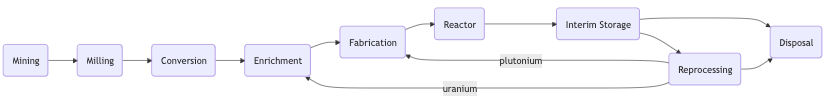
\includegraphics[scale=0.55]{images/nfc/closed_fc.png}
      \caption{Hypothetical closed fuel cycle.}
      \label{fig:closed_fc}
\end{figure}


\subsection{Front End of the Fuel Cycle}
\label{sec:front_end}
At the time of writing, the \gls{nea} and \gls{iaea} have not released their  2024 \textit{Red Book}; however, interested parties can extrapolate trends from the 2022 \textit{Red Book} report on global Uranium availability, which covers January 2019 to January 2021 and updates the projections from 54 countries of their uranium supply and resources through 2040 \cite{nea_red_book_2022}.

Globally, Australia holds the most significant reasonably assured resources
of uranium at roughly 28\% of the world's total. However, total identified recoverable resources declined 2\% from 2019 to 2021--in contrast with slight increases reported in previous versions of the report--as countries increased mining efforts, reclassified economic viability of inferred resources, and currency values fluctuated with inflation. Among the most well-established uranium exporters like Australia, Canada, and Kazakhstan re-evaluations of inferred resources accounted for decreases in nearly every quality category, while relatively new exporters, Mongolia and Niger, reported increases in inferred resources \cite{nea_red_book_2022}. This thesis focuses on the \gls{usa} explicitly and does not incorporate geospatial information.

The \gls{usa} imports more uranium than it produces domestically, as shown in Figure \ref{fig:foregin_u3o8}, from countries with large uranium deposits like Canada, Australia, and Kazakhstan. This trend is expected to continue as the \gls{usa} has only recently begun to invest in new uranium mines since the 1980s.

\begin{figure}[H]
   \centering
   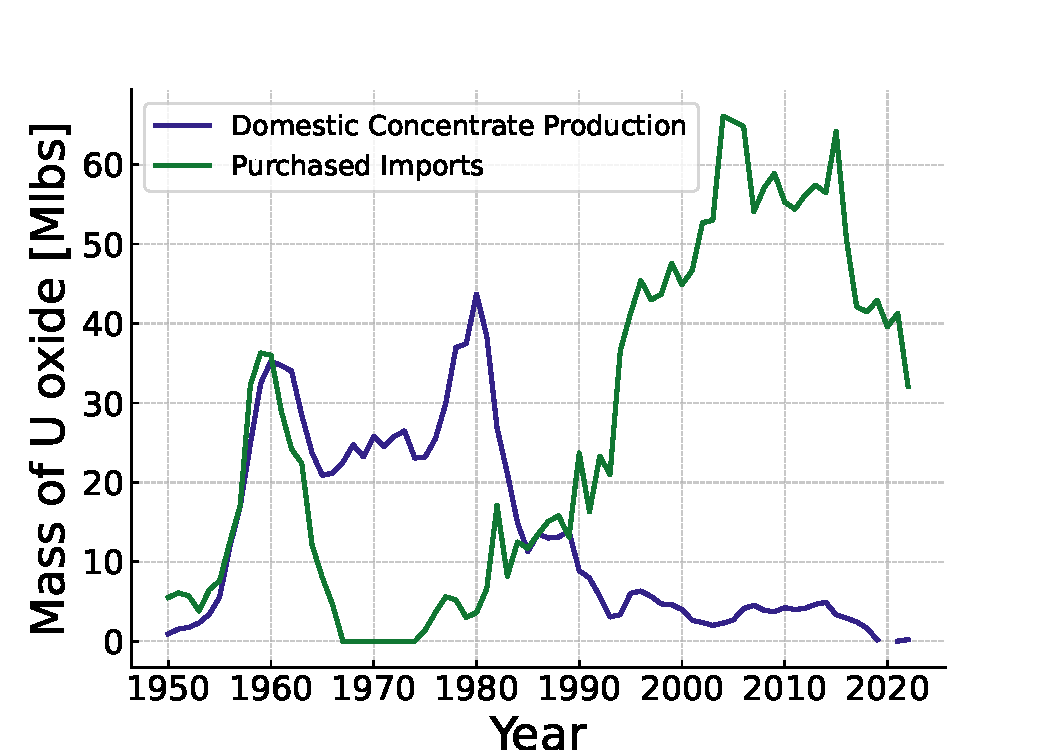
\includegraphics[scale=0.7]{images/intro/uranium_production_imports.pdf}
   \caption{Foreign and domestic uranium purchases over time. Reproduced from \cite{eia_monthly_energy_review_2024}.}
   \label{fig:foregin_u3o8}
\end{figure}

As the 2022 \textit{Red Book} notes, the literature surrounding the understanding of best practices for environmental stewardship and remediation of mines is growing. Once-common practices of strip, pit, and underground
mining are beginning to be replaced with more sustainable practices that
minimize the environmental impact of mining. One method that has garnered
interest in the uranium mining community is in-situ leaching, wherein automatic pumps inject a leaching solution into the ground to dissolve the uranium and then pump the solution to the surface for processing \cite{insitu_review_2024}. In-situ leaching is limited to areas with favorable permeabilities, but the reduced labor intensity, simplified infrastructure requirements, and lower environmental impact make it an attractive option for uranium mining where applicable.

In-situ leaching also reduces the extent of the milling process as the ratio of
desirable material to non-desirable material is higher in the leaching solution
than in the resultant material from traditional mining. The milling process
generally involves crushing the ore into a fine powder and then leaching the
uranium from the ore with a sulfuric acid solution. Workers then extract the
uranium from the solution and convert it into yellowcake ($U_3O_8$), a
concentrated form of uranium oxide \cite{milling_uranium_2022}. The yellowcake
is then shipped to a conversion facility, where it is converted into uranium
hexafluoride ($UF_6$), a gas that cools to a liquid and then a solid before it
is transported to be enriched. Uranium hexafluoride is attractive in the
enrichment process because fluorine has only one naturally occurring isotope
and is easy to ensure isolation from the uranium.

Up to the enrichment stage of the fuel cycle, the process is almost entirely
agnostic to the end use of the uranium fuel. Leaving the conversion stage,
$UF_6$ enters the enrichment process aims to achieve a specific concentration
or weight percent of $^{235}$U relative to the other uranium isotopes. Today,
enrichment relies on centrifuges, which separate the isotopes based on their
mass; however, historical gaseous diffusion technology could potentially use
laser enrichment if it becomes economically viable. This thesis does not
distinguish between enrichment services; instead, using \gls{swu}, which Section
\ref{sec:swu} expands on, to quantify the enrichment delivered.

The enriched $UF_6$ is then converted into uranium dioxide ($UO_2$) and
fabricated into fuel. For the \gls{usa} fleet of large \glspl{lwr}, the fuel is made into pellets, stacked into rods, and collected into assemblies. This is not the case for every reactor design, as some reactors use prismatic, pebble, or liquid fuel elements. As with enrichment, the fabrication stage of the fuel cycle is simplified in this thesis, and this thesis does not incorporate explicit details of the fabrication process.

\subsection{Reactor Operation}
\label{sec:reactor_operation}
Up to now, this section has laid out the front end of the fuel cycle. The part of the \gls{nfc} where the fuel is used in the reactor is neither at the front nor back of the fuel cycle. Inside the reactor core, the fuel generates heat through fission, which produces steam, thereby driving a turbine to generate electricity. The fuel remains in the reactor for several years, depending on the reactor design and fuel enrichment. % This interstitial phase of the \gls{nfc} is now complete.


\subsection{Back-End of the Fuel Cycle}
\label{sec:back_end}
% used fuel storage
After the fuel has been in the reactor for several years, it is removed and
stored in a spent fuel pool. After cooling, the fuel is moved to dry cask
storage, where it will remain until a long-term solution is implemented.
This thesis does not focus on closed-fuel cycles, therefore it does not consider fuel reprocessing in this description of the \gls{nfc}.

% How is radioactive waste managed and disposed of?
When considering a long-term repository for the used fuel, maintainers must consider the macroscopic and microscopic effects of the environment on the repository. On a macroscopic level, climate change will drive shoreline erosion, permafrost recession, and congenital ice sheet melting. Translating these well-known effects into chemical consequences that dictate the design of a repository will require site-specific adaptations on several fronts. Special attention must be given to the impact in the first few thousand years, as this period will exhibit the highest activity. In the case of meltwater exposure, water saturated with dissolved $O_2$ could infiltrate a repository, potentially altering the oxidizing conditions \cite{gurban_hydrochemical_2001}. Consequently, regulators considering the 100,000-year perspective of a potential repository must account for proximity to such meltwater sources to meet the demands imposed by a changing climate.

Sites experiencing reducing conditions may continue to do so; however, the changing climate will also influence the salinity of groundwater. Changes in salinity affect density, which could either exacerbate or mitigate the spread of contaminants in the event of exposure outside the repository \cite{gurban_hydrochemical_2001}. This change in salinity also has the potential to interact differently with canisters, necessitating that proactive regulators ensure containment is designed to withstand a changing environment over the repository's lifetime.

An additional layer of microscopic consideration for these regulatory concerns
is the imminent deployment of new nuclear fuels with different compositions and
forms. Some fuels are designed with pyrolytic carbon matrices that can
immobilize decay products for much longer than current fuel forms. As new fuel
technologies are deployed, \gls{nfc} facilities will adapt accordingly. These changes, although seemingly slight (the fuel will likely still be uranium-based), can have significant consequences over 100,000 years
of storage \cite{hyland_post_closure_2013}.